El objetivo de esta gu\'{\i}a de usuario es proporcionar a los usuarios un ejemplo para la puesta a punto y ejecuci\'on de las 
funcionalidades implementadas en el gema RuQL durante el Trabajo de Fin de Grado.

%---------------------------------------------------------------------------------
\section{Instalaci\'on de la gema}
\label{Apendice2:instalacion}

Para instalar la \ceit{gema}, basta con ejecutar el siguiente comando:
\begin{verbatim}
[~]$ gem install ruql
\end{verbatim}

Si deseamos ejecutar la gema sin instalarla, debemos hacer lo siguiente:
\begin{itemize}
  \item Descargar el c\'odigo desde \href{https://github.com/jjlabrador/ruql}{\ceit{GitHub}}.
  \item Ejecutar el siguiente comando desde la ra\'{\i}z del proyecto:
  \begin{verbatim}
  [~]$ ruby -Ilib bin/ruql [argumentos]
  \end{verbatim}
\end{itemize}

Tambi\'en se puede instalar la gema a partir del c\'odigo fuente y no usando el repositorio de gemas de \ceit{Ruby}. Una vez descargado el c\'odigo, ejecutamos los siguientes
comandos:
\begin{verbatim}
[~ruql]$ gem build ruql.gemspec
\end{verbatim}
Este comando nos crear\'a el paquete de la gema listo para instalar usando:
\begin{verbatim}
[~ruql]$ gem install ./ruql-0.0.5.gem
\end{verbatim}
\newpage

Como el repositorio cuenta con un \ceit{Rakefile}, podemos ejecutar la siguiente tarea de \ceit{Rake} que automatiza los comandos descritos anteriormente:
\begin{verbatim}
[~ruql]$ rake install
\end{verbatim}

Este Rakefile, adem\'as, cuenta con numerosas tareas \'utiles para la generaci\'on de cuestionarios.
\bigskip

{\bfseries NOTA}: a falta de que se lleve a cabo el \cei{Pull-Request}, la instalaci\'on de la gema a partir del c\'odigo fuente es la \'unica manera de tener la \'ultima versi\'on
de RuQL.
\bigskip

Para consultar la ayuda sobre qu\'e argumentos opcionales recibe cada \ceit{renderer}, basta con escribir lo siguiente:
\begin{verbatim}
[~]$ ruql --help
\end{verbatim}
si tenemos la gema instalada en nuestra m\'aquina o
\begin{verbatim}
[~]$ ruby -Ilib bin/ruql --help
\end{verbatim}
si la ejecutamos desde el c\'odigo fuente.
\bigskip

Entre ellos destacan las opciones de a\~{n}adir hojas de estilo (\textit{-c}), JavaScripts (\textit{-j}) y especificar un propio \ceit{template} (\textit{-t}) de \ceis{\ref{apend1:erb}}.
Si se desea emplear un template propio, \'este debe contener una serie de variables obligatoriamente para que se inserten los recursos necesarios y el renderer funcione
correctamente. A continuaci\'on se muestra un ejemplo de template con dichas variables necesarias. Adem\'as, ser\'a posible a\~{n}adirle un \ceit{header} y un \ceit{footer} personalizado. 
De este modo no ser\'{\i}a necesario elaborar un template completamente nuevo cada vez. Para ello basta con indicarlo en nuestro fichero Ruby. Los m\'etodos \textit{head} y
\textit{foot} admiten tanto un path (escrito como un \ceis{s\'{\i}mbolo}) de donde se encuentre el \ceit{c\'odigo} \ceit{HTML} o un {\bfseries string} con el propio HTML:

\begin{verbatim}
<html>
  <head>
    <meta charset="utf-8">
    <meta http-equiv="X-UA-Compatible" content="IE=edge">
    <meta name="viewport" content="width=device-width, initial-scale=1">
    <title><%= quiz.title %></title>
    <!-- Bootstrap CSS -->
    <%= @bootstrap_css %>
    <style type="text/css" media="all">
      /* Custom CSS */
      /* ...........*/
      /* Inputs size */
      <%= @sass %>
    </style>
    <!-- jQuery ContextMenu CSS -->
    <%= @context_menu_css %>
    <!-- Any CSS included by the user -->
    <%= @css_custom %>
    <!-- Mathjax -->
    <%= @mathjax %>
    <!-- CodeMirror -->
    <%= @codemirror %>
  </head>
  <body>
   <div class="container">
      <% if (quiz.get_header)%>
          <h3><%= quiz.title %></h3>
          <%= quiz.get_header %>
          <br></br>
      <% else %>
        <!-- HTML Code -->
      <% end %>
      <%= yield %>
      <% if (quiz.get_footer) %>
        <%= quiz.get_footer %>
        <br></br>
      <% else %>
        <!-- HTML Code -->
      <% end %>
    </div>
    <!-- #### JavaScripts #### -->
    <!-- jQuery -->
    <%= @jQuery %>
    <!-- Internationalization -->
    <%= @i18n %>
    <!-- Drag and Drop -->
    <%= @dragdrop %>
    <!-- XRegexp -->
    <%= @xregexp %>
    <!-- Form validation -->
    <%= @validation_js %>
    <!-- jQuery ContextMenu -->
    <%= @context_menu %>
    <!-- Any JavaScript included by the user -->
    <%= @js_custom %>
    <!-- CodeMirror object -->
    <%= @codemirror_object %>
    <!-- JavaScript for Bootstrap -->
    <%= @bootstrap_js %>
  </body>
</html>
\end{verbatim}

Si no se especifica template, se mostrar\'a un HTML sin apenas estilo. El profesor se deber\'a encargar de adecuarlo a su gusto posteriormente. 

%---------------------------------------------------------------------------------
%---------------------------------------------------------------------------------
\section{HtmlForm renderer}
\label{Apendice2:htmlform}

A continuaci\'on veremos un ejemplo de \ceit{cuestionario} explicando las peculiaridades de cada tipo de pregunta:

El fichero \ceit{Ruby} debe comenzar de esta manera:
\begin{lstlisting}
quiz 'Example quiz' do
  head :'examples/header.html'  # Opcional
  
  # Preguntas
  
  foot :'examples/footer.html'  # Opcional
end
\end{lstlisting}
\bigskip

%---------------------------------------------------------------------------------
\subsection{Preguntas \ceit{FillIn}}
\label{subsec:Apendice2.1}

Para que el \ceit{renderer} genere las etiquetas \ceit{input}, se deben especificar tres guiones ('-') como m\'{\i}nimo. Si la cantidad es menor que tres, se mostrar\'an los guiones
en el cuestionario. Si queremos que se muestren m\'as de tres guiones seguidos, debemos escaparlos. Recuerda adem\'as que el n\'umero de guiones establecer\'a el largo del input.
\begin{lstlisting}
tag = '<a href="www.google.es"></a> '
fill_in do
  text "<i>Example of escaped HTML and three hyphens not evaluated:</i><br> 
  #{escape(tag)}" + "is a \\-\\-\\- ---- " + '\-\-\-'
  answer /^link$/
end
\end{lstlisting}
\bigskip

Ejemplo de pregunta con un \cei{distractor} y un comentario:
\begin{lstlisting}
fill_in :points => 2 do
  text 'The visionary founder of Apple is --------'
  comment 'Question too easy'
  answer /^ste(ve|phen)\s+jobs #comment $/imx
  distractor /^steve\s+wozniak/i, :explanation => 'Almost, but not quite.'
end
\end{lstlisting}
\newpage

Ejemplo de pregunta con c\'odigo \ceit{LaTeX}:
\begin{lstlisting}
fill_in do
  text %q{
    When x = 2, the solution of $\sqrt{3x+3}+(1+x)^2$ is:
    ----
  }
  answer 12
  distractor 11, :explanation => "Try again!"
end
\end{lstlisting}
\bigskip

La respuesta a la pregunta puede ser una cadena, una expresi\'on regular, un n\'umero o un objeto \ceit{JavaScript}. En el caso de los tres primeros tipos de respuesta, se usar\'a
un \cei{Array} si hay m\'as de una respuesta en la pregunta.
\begin{lstlisting}
fill_in do
  text 'The ---- brown fox jumped over the lazy ----'
  answer [/fox/, /dog/]
end
\end{lstlisting}
\bigskip

Se puede usar la opci\'on \textit{order} para especificar si las respuestas dadas se corresponden con el orden dado en la pregunta. Por defecto est\'a a {\bfseries true}.
\begin{lstlisting}
fill_in do
  text 'The ---- brown fox jumped over the lazy ----'
  answer [/fox/, /dog/], :order => false
end
\end{lstlisting}

{\bfseries NOTA}: en caso de especificar en el Array dos respuestas iguales para dos huecos diferentes, forzosamente es necesario especificar \textit{order} a {\bfseries true}.
\bigskip

Tambi\'en se pueden escribir este tipo de preguntas de dos formas m\'as compactas:
\bigskip

Esta primera forma permite colocar la respuesta al lado de los guiones. S\'olo se admiten respuestas de tipo \cei{String}.
\begin{lstlisting}
fill_in do
  text 'The three stooges are -----{larry}, ----{moe}, and -----{curly}.'
end
\end{lstlisting}
\bigskip

Esta otra forma permite asociar las respuestas con una clave, que la definiremos en un \ceis{Hash} que se pasar\'a como respuesta.
\begin{lstlisting}
fill_in do
  text "The capital of Tenerife is -----{:santa} Cruz de --------{:tenerife}"
  answer :santa => /Santa/i, :tenerife => /Tenerife/i
end
\end{lstlisting}
\bigskip

Por \'ultimo, tenemos las respuestas de tipo {\bfseries objeto JavaScript}. La opci\'on \textit{order} debe ser siempre {\bfseries true}:
\begin{lstlisting}
fill_in do
  text %q{
    Diga dos numeros x = ---- e  y = ---- que multiplicados den 100
  }
  answer JavaScript.new(%q{result = function(x,y) { return (x * y === 100); }})
end
\end{lstlisting}

%---------------------------------------------------------------------------------
\subsection{Preguntas \ceit{Drag and Drop} FillIn}
\label{subsec:Apendice2.2}

Son muy similares a las preguntas FillIn normales. S\'olo admiten respuestas de tipo \textit{String} pero admiten los mismos par\'ametros opcionales.
\begin{lstlisting}
drag_drop_fill_in do
  text 'The ---- brown fox jumped over the lazy ----'
  answer ['fox', 'dog']
end
\end{lstlisting}

%---------------------------------------------------------------------------------
\subsection{Preguntas \ceit{Multiple Choice}}
\label{subsec:Apendice2.3}

Aqu\'{\i} se presenta un ejemplo de este tipo de pregunta. Usando la opci\'on \textit{randomize}, el renderer ordenar\'a al azar todas las respuestas
y el cuestionario generado las mostrar\'a en diferente orden:
\begin{lstlisting}
choice_answer :randomize => true do
  text  "What is the largest US state?"
  explanation "Not big enough." # for distractors without their own explanation
  answer 'Alaska'
  distractor 'Hawaii'
  distractor 'Texas', :explanation => "That's pretty big, but think colder."
end
\end{lstlisting}

%---------------------------------------------------------------------------------
\subsection{Preguntas TrueFalse}
\label{subsec:Apendice2.4}

\'Este es un caso particular de las preguntas {\bfseries Multiple Choice}:
\begin{lstlisting}
truefalse 'The earth is flat.', false, :explanation => 'No, just looks that way'
\end{lstlisting}
\newpage

%---------------------------------------------------------------------------------
\subsection{Preguntas Drag and Drop Multiple Choice}
\label{subsec:Apendice2.5}

Para las preguntas Multiple Choice de Drag and Drop no hace falta especificar la opci\'on \textit{randomize}, el \ceit{renderer} cambiar\'a el orden de las 
respuestas siempre.
\begin{lstlisting}
drag_drop_choice_answer do
  text  "Relate these concepts"
  relation :Facebook => 'Mark Zuckerberg', :Twitter => 'Jack Dorsey'
end
\end{lstlisting}

%---------------------------------------------------------------------------------
\subsection{Preguntas Select Multiple}
\label{subsec:Apendice2.6}

Las preguntas de \ceit{Select Multiple} se definen del siguiente modo:
\begin{lstlisting}
select_multiple do
  text "Which are American political parties?"
  answer "Democrats"
  answer "Republicans"
  answer "Greens", :explanation => "Yes, they're a party!"
  distractor "Tories", :explanation => "They're British"
  distractor "Social Democrats"
end
\end{lstlisting}

%---------------------------------------------------------------------------------
\subsection{Preguntas Drag and Drop Select Multiple}
\label{subsec:Apendice2.7}

Para las preguntas de Drag and Drop Select Multiple basta con especificar lo siguente:
\begin{lstlisting}
drag_drop_select_multiple do
  text  "Relate these concepts"
  relation :Ruby => ['Sinatra', 'Rails'], :JavaScript => 'jQuery'
end
\end{lstlisting}

Se deber\'a usar una notaci\'on de \ceis{Array} cuando haya m\'ultiples respuestas para un determinado item. Cuando s\'olo exista una respuesta por item,
se puede indicar como un \ceis{String}.

%---------------------------------------------------------------------------------
\subsection{Preguntas Programming}
\label{subsec:Apendice2.8}

Para las preguntas de tipo \ceis{Programming} se puede especificar diversos par\'ametros:
\begin{itemize}
  \item El lenguaje. Como este renderer valida las respuestas mediante \ceit{JavaScript}, s\'olo se permite este lenguaje.
  \item Ancho y largo. Si no se especifica, el cuadro de texto para redactar la respuesta ser\'a de 150px de largo y 800px de ancho.
\end{itemize}

{\bfseries NOTA}: el par\'ametro \textit{order} siempre debe ser {\bfseries true}. Est\'a configurado para ello por defecto.
\bigskip
\bigskip

Para la respuesta, se puede especificar: 
\begin{itemize}
  \item Un path indicando donde est\'a el fichero que testea la respuesta introducida por el alumno: para ello, es necesario expresar ese path como un \ceis{s\'{\i}mbolo}.
  \item Escribir como un {\bfseries String} el c\'odigo JavaScript que testea la entrada del alumno.
\end{itemize}
\bigskip

A continuaci\'on se muestra un ejemplo especificando un path donde se encuentra el fichero JavaScript con el que se comprueba la respuesta introducida del alumno:
\begin{lstlisting}
programming :language => 'JavaScript', :height => 150, :width => 800  do
  text %q{Write a JavaScript function named `suma` with two arguments that
  return the sum of them}
  answer JavaScript.new(:'examples/test_suma.js')
end
\end{lstlisting}

%---------------------------------------------------------------------------------
\subsection{Otras consideraciones}
\label{subsec:Apendice2.9}

\begin{itemize}
  \item Todas las respuestas se guardar\'an una vez pulsado el bot\'on de \textit{enviar} haciendo uso de \ceis{Local Storage}. Para cada cuestionario generado, habr\'a 
  un objeto guardado dentro de Local Storage. Es recomendable borrar el almacenamiento frecuentemente para que no persista en el navegador.
  \item EL men\'u contextual que muestra las respuestas s\'olo funciona en preguntas de tipo {\bfseries FillIn} cuyas respuestas sean \textit{Strings}, \cei{RegExp} o num\'ericas.
  Para las preguntas de tipo test existe un bot\'on que muestra y oculta las respuestas correctas.
\end{itemize}

%---------------------------------------------------------------------------------
\subsection{Generando el cuestionario}
\label{subsec:Apendice2.10}

Para generar el cuestionario, ejecutamos el siguiente comando:
\begin{verbatim}
[~]$ ruql [ruta_fichero_rb] HtmlForm -t [ruta_template.html.erb] > [fichero_salida].html
\end{verbatim}
\newpage

%---------------------------------------------------------------------------------
%---------------------------------------------------------------------------------
\section{Sinatra renderer}
\label{Apendice2:sinatra}

Este renderer permite todas los tipos de preguntas mencionados anteriormente con la diferencia de que en las preguntas de c\'odigo (\cei{FillIn} y \cei{Programming}), 
el lenguaje permitido es \ceis{Ruby}. A continuaci\'on veremos dos ejemplos:

%---------------------------------------------------------------------------------
\subsection{Preguntas FillIn}
\label{subsec:Apendice2.11}

\begin{lstlisting}
fill_in do
  text %q{
    Diga dos numeros x = ---- e  y = ---- que multiplicados den 100
  }
  answer Ruby.new(%q{Proc.new do |x,y| x * y == 100 end})
end
\end{lstlisting}

%---------------------------------------------------------------------------------
\subsection{Preguntas Programming}
\label{subsec:Apendice2.11}

\begin{lstlisting}
programming :language => 'Ruby', :height => 150, :width => 800  do
  text %q{Write a Ruby function named `suma` with two arguments that 
  return the sum of them}
  answer Ruby.new(:'examples/test_suma.rb')
end
\end{lstlisting}

%---------------------------------------------------------------------------------
\subsection{Par\'ametros adicionales}
\label{subsec:Apendice2.12}

En el fichero Ruby que recibe como entrada la gema, adem\'as de definir las preguntas, se debe especificar a los usuarios que har\'an
uso de la aplicaci\'on:

\begin{itemize}
  \item Por un lado, se deben indicar a los profesores que podr\'an desplegar el examen o consultar las notas de los alumnos. Se indicar\'a
  su email de Google en forma de \cei{string}. En caso de ser m\'ultiples profesores, se usar\'a una notaci\'on de \cei{array}. 
  \begin{lstlisting}
  quiz 'Example quiz' do
    
    teachers 'jjlabradorglez@gmail.com'
    
    .
    .
    .
  end
  \end{lstlisting}
  
  \item Por otra parte, se deber\'an indicar los alumnos permitidos para realizar el cuestionario. Se puede usar un \cei{Hash} con 
  la informaci\'on necesaria de ellos. 
  \begin{lstlisting}
  quiz 'Example quiz' do
    
    students :'jjlabradorglez@gmail.com' => {:surname => 'Labrador Gonzalez', 
               :name => 'Juan Jose'}, 
             :'tutu@gmail.com' => {:surname => 'Chuchu', :name => 'Tutu'}
    .
    .
    .
  end
  \end{lstlisting}
  
  O indicar el path de un fichero \ceis{CSV} con los datos de los mismos llamado \textit{students.csv}.
  \begin{lstlisting}
  quiz 'Example quiz' do
    
    students :'examples/students.csv''
    
    .
    .
    .
  end
  \end{lstlisting}
  
  El formato del fichero CSV debe ser del siguiente modo:
  \begin{verbatim}
  casiano.rodriguez.leon@gmail.com, Rodriguez Leon, Casiano
  tutu@gmail.com, Chuchu, Tutu
  youwapp@gmail.com, Developers, YouWapp
  \end{verbatim}
  
\end{itemize}

Adem\'as, es necesario especificar un fichero \textit{config.yml} que contiene la ventana temporal en la cual estar\'a disponible
el cuestionario, el nombre del subdominio de Heroku que se desea usar para desplegar el cuestionario y la informaci\'on relativa a \ceit{Google Drive}:
\begin{itemize}
  \item Nombre de la hoja de c\'alculo donde se guardar\'an los datos de alumnos y preguntas y respuestas.
  \item Nombre de la carpeta que contendr\'a dicha \ceit{hoja de c\'alculo}.
  \item Path donde queremos que se cree la carpeta y la hoja de c\'alculo (si no existe alguna carpeta del path, se crear\'a tambi\'en).
  \item \ceit{API} keys necesarias para poder usar los servicios de Google, tanto la autenticaci\'on con OAuth como la escritura en Google Drive. 
  En la siguiente subsecci\'on,  se indicar\'an los pasos a realizar para dar de alta una aplicaci\'on en \ceis{Google Developers Console}.
\end{itemize}

{\bfseries NOTA}: el nombre del subdominio de \ceit{Heroku} solo puede contener letras y n\'umeros. Tampoco puede contener espacios. Sin embargo, puede especificarse
con espacios en el fichero \textit{config.yml}, el renderer lo modificar\'a para que Heroku lo acepte.
\bigskip

\begin{figure}[!th]
\begin{center}
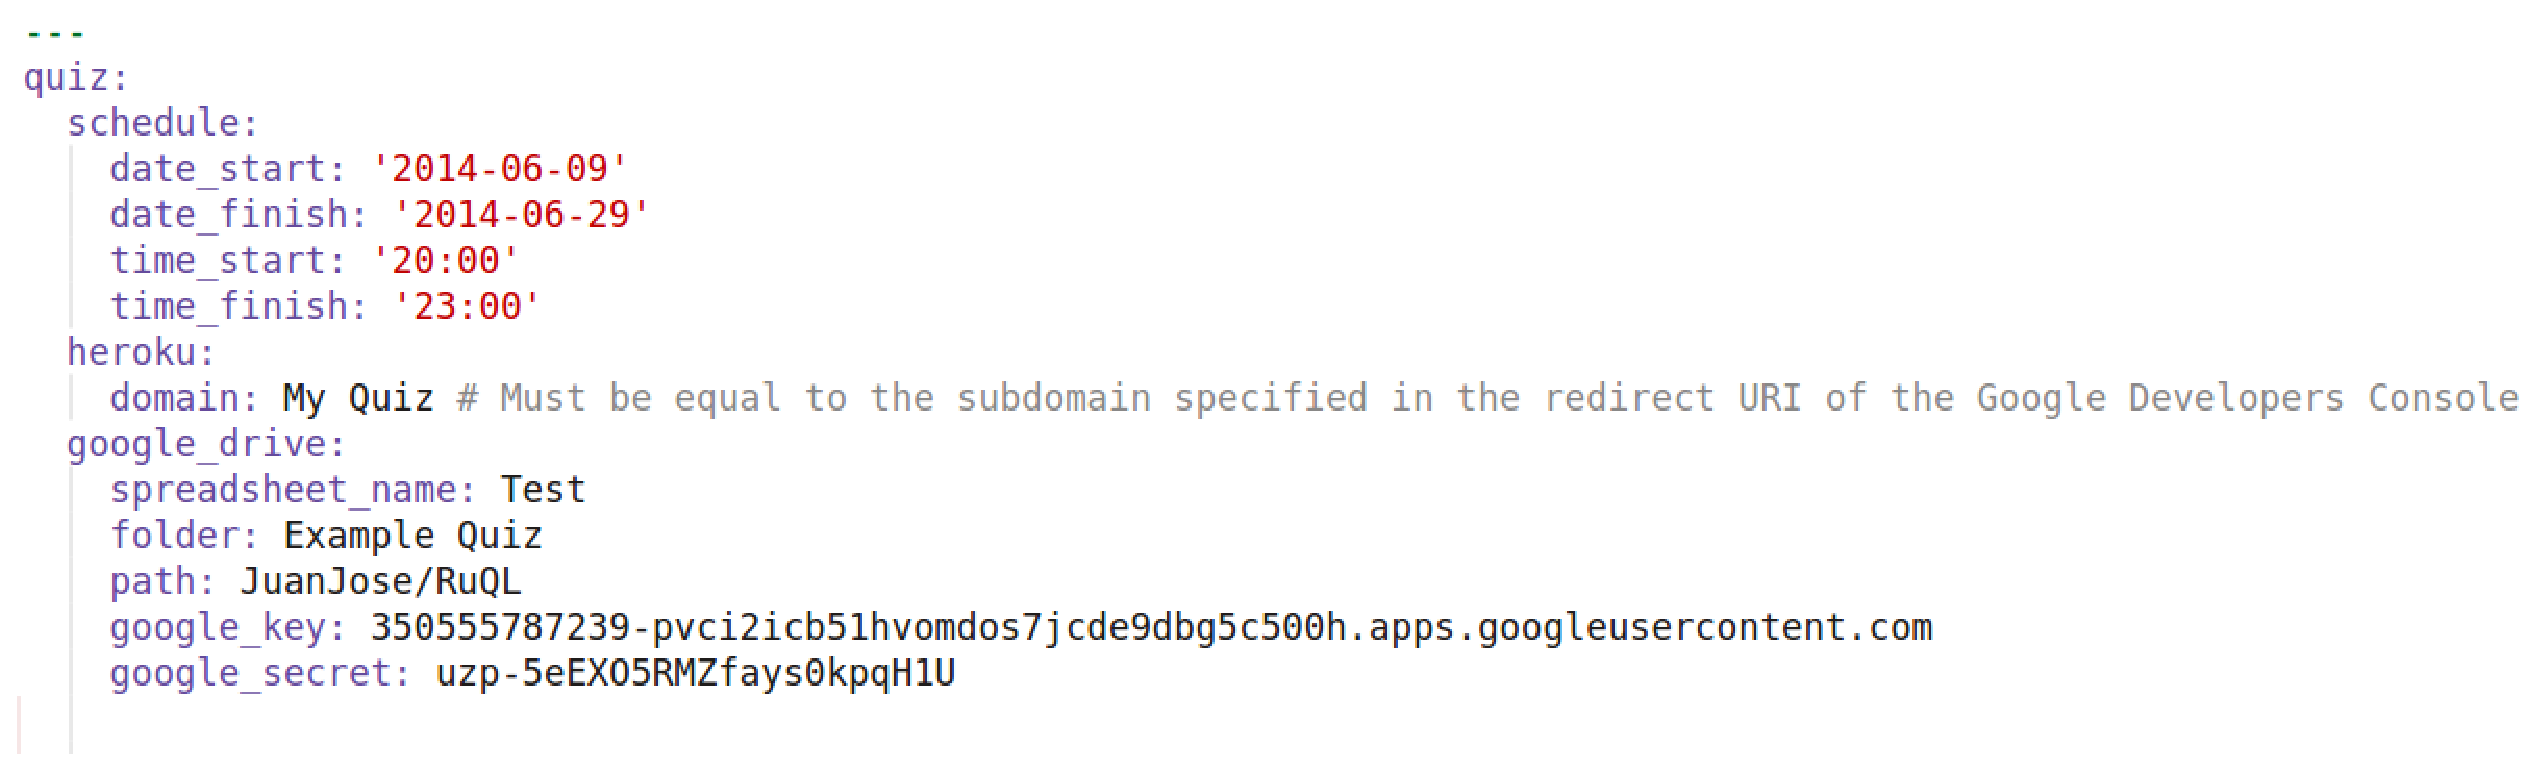
\includegraphics[width=1.2\textwidth]{images/config_yml.eps}
\caption{Ejemplo de fichero \textit{config.yml} con la informaci\'on necesaria}
\label{fig:config_yml}
\end{center}
\end{figure}
\newpage

Para a\~{n}adir este fichero al fichero del cuestionario especificamos el path del fichero en notaci\'on de \ceis{s\'{\i}mbolo}:
\begin{lstlisting}
  quiz 'Example quiz' do
    
    .
    .
    
    config :'examples/config.yml'
    .
    .
  end
\end{lstlisting}
\newpage

%---------------------------------------------------------------------------------
\subsection{Dar de alta una aplicaci\'on en Google Developers Console}
\label{subsec:Apendice2.13}

Pasos para dar de alta una aplicaci\'on en \ceit{Google Developers Console}:
\begin{enumerate}
  \item Dirigirse a \href{https://console.developers.google.com/}{Google Developers Console}
  
  \item Crear un nuevo proyecto.
  \begin{figure}[H]
  \begin{center}
  
\includegraphics[width=0.5\textwidth]{images/gdc0.eps}
  \caption{Bot\'on para crear un nuevo proyecto}
  \label{fig:gdc0}
  \end{center}
  \end{figure}
  
  \item Elegir un nombre para el proyecto.
  \begin{figure}[!th]
  \begin{center}
  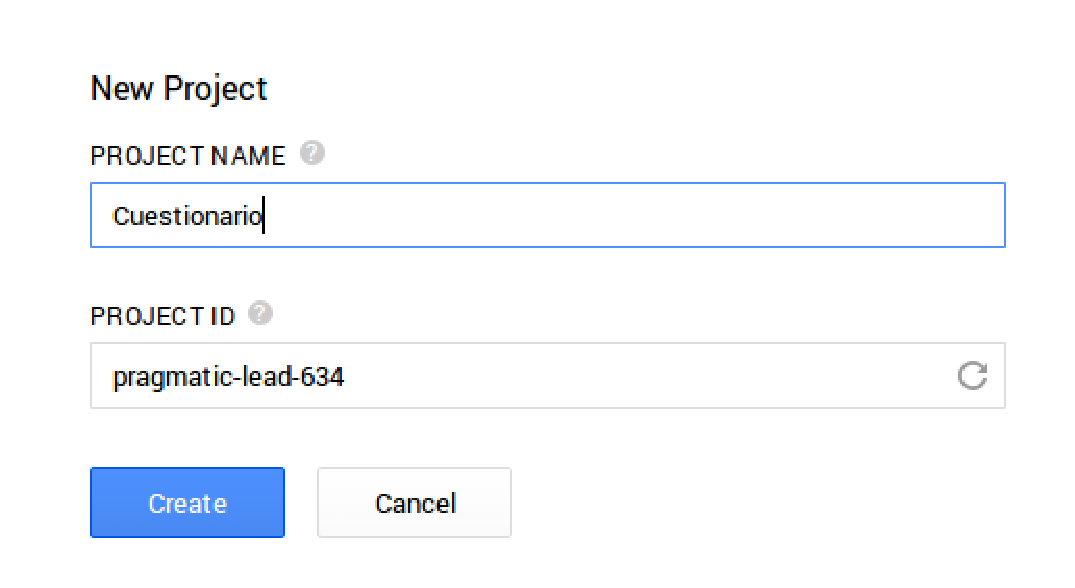
\includegraphics[width=0.7\textwidth]{images/gdc1.eps}
  \caption{Elegir nombre para el proyecto}
  \label{fig:gdc1}
  \end{center}
  \end{figure}
  \newpage
  
  \item Una vez se ha creado, se nos redireccionar\'a al mismo. Pinchamos en la secci\'on {\bfseries APIS \& AUTH} y elegimos la opci\'on \textit{APIs}.
  \begin{figure}[!th]
  \begin{center}
  
\includegraphics[width=0.3\textwidth]{images/gdc2.eps}
  \caption{Apartado de APIs}
  \label{fig:gdc2}
  \end{center}
  \end{figure}
    
  Deberemos activar las siguientes APIs:
  \begin{enumerate}
    \item \textit{Contacts API}
    \item \textit{Drive API}
    \item \textit{Drive SDK}
    \item \textit{Google+ API}
  \end{enumerate}
  \newpage
  
  \item Una vez hecho esto, nos iremos al apartado \textit{Credentials} dentro de {\bfseries APIS \& AUTH} y seleccionaremos \textit{Create new Client ID}.
  \begin{figure}[!th]
  \begin{center}
  
\includegraphics[width=0.3\textwidth]{images/gdc3.eps}
  \caption{Apartado de credenciales}
  \label{fig:gdc3}
  \end{center}
  \end{figure}
  
  \begin{figure}[!th]
  \begin{center}
  
\includegraphics[width=0.5\textwidth]{images/gdc4.eps}
  \caption{Crear nuevo cliente ID}
  \label{fig:gdc4}
  \end{center}
  \end{figure}
  \newpage
  
  \item Seleccionamos \textit{Web application} y establecemos la \ceit{URI} a la que \ceit{Google} debe devolvernos los datos. La URI debe ser igual a la de la imagen salvo
  en el subdominio de \ceit{Heroku}, en el que pondremos el que nos ha dado Heroku o el que hemos especificado en nuestro \textit{config.yml}
  \begin{figure}[!th]
  \begin{center}
  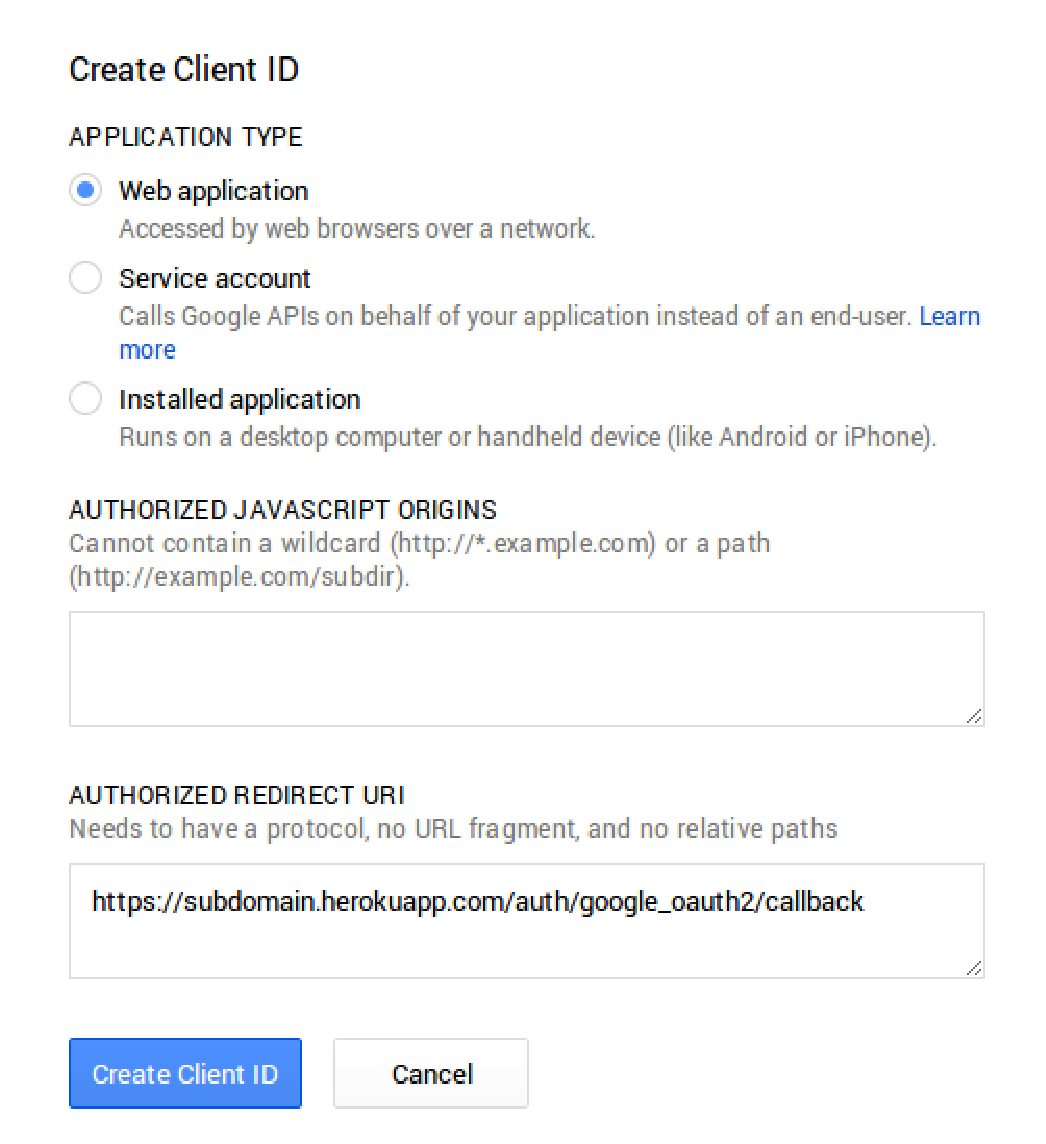
\includegraphics[width=0.7\textwidth]{images/gdc5.eps}
  \caption{Pantalla de creaci\'on del cliente ID}
  \label{fig:gdc5}
  \end{center}
  \end{figure}
  \newpage
  
  \item Opcionalmente, nos podemos dirigir al apartado \textit{Consent screen} dentro de {\bfseries APIS \& AUTH} para indicar el nombre que queremos que aparezca
  en la pantalla de permisos cuando alguien vaya a dar permiso a nuestra aplicaci\'on para que use sus datos. Adem\'as, se pueden a\~{n}adir otros campos tales como
  logos, URLs, etc.
  \begin{figure}[!th]
  \begin{center}
  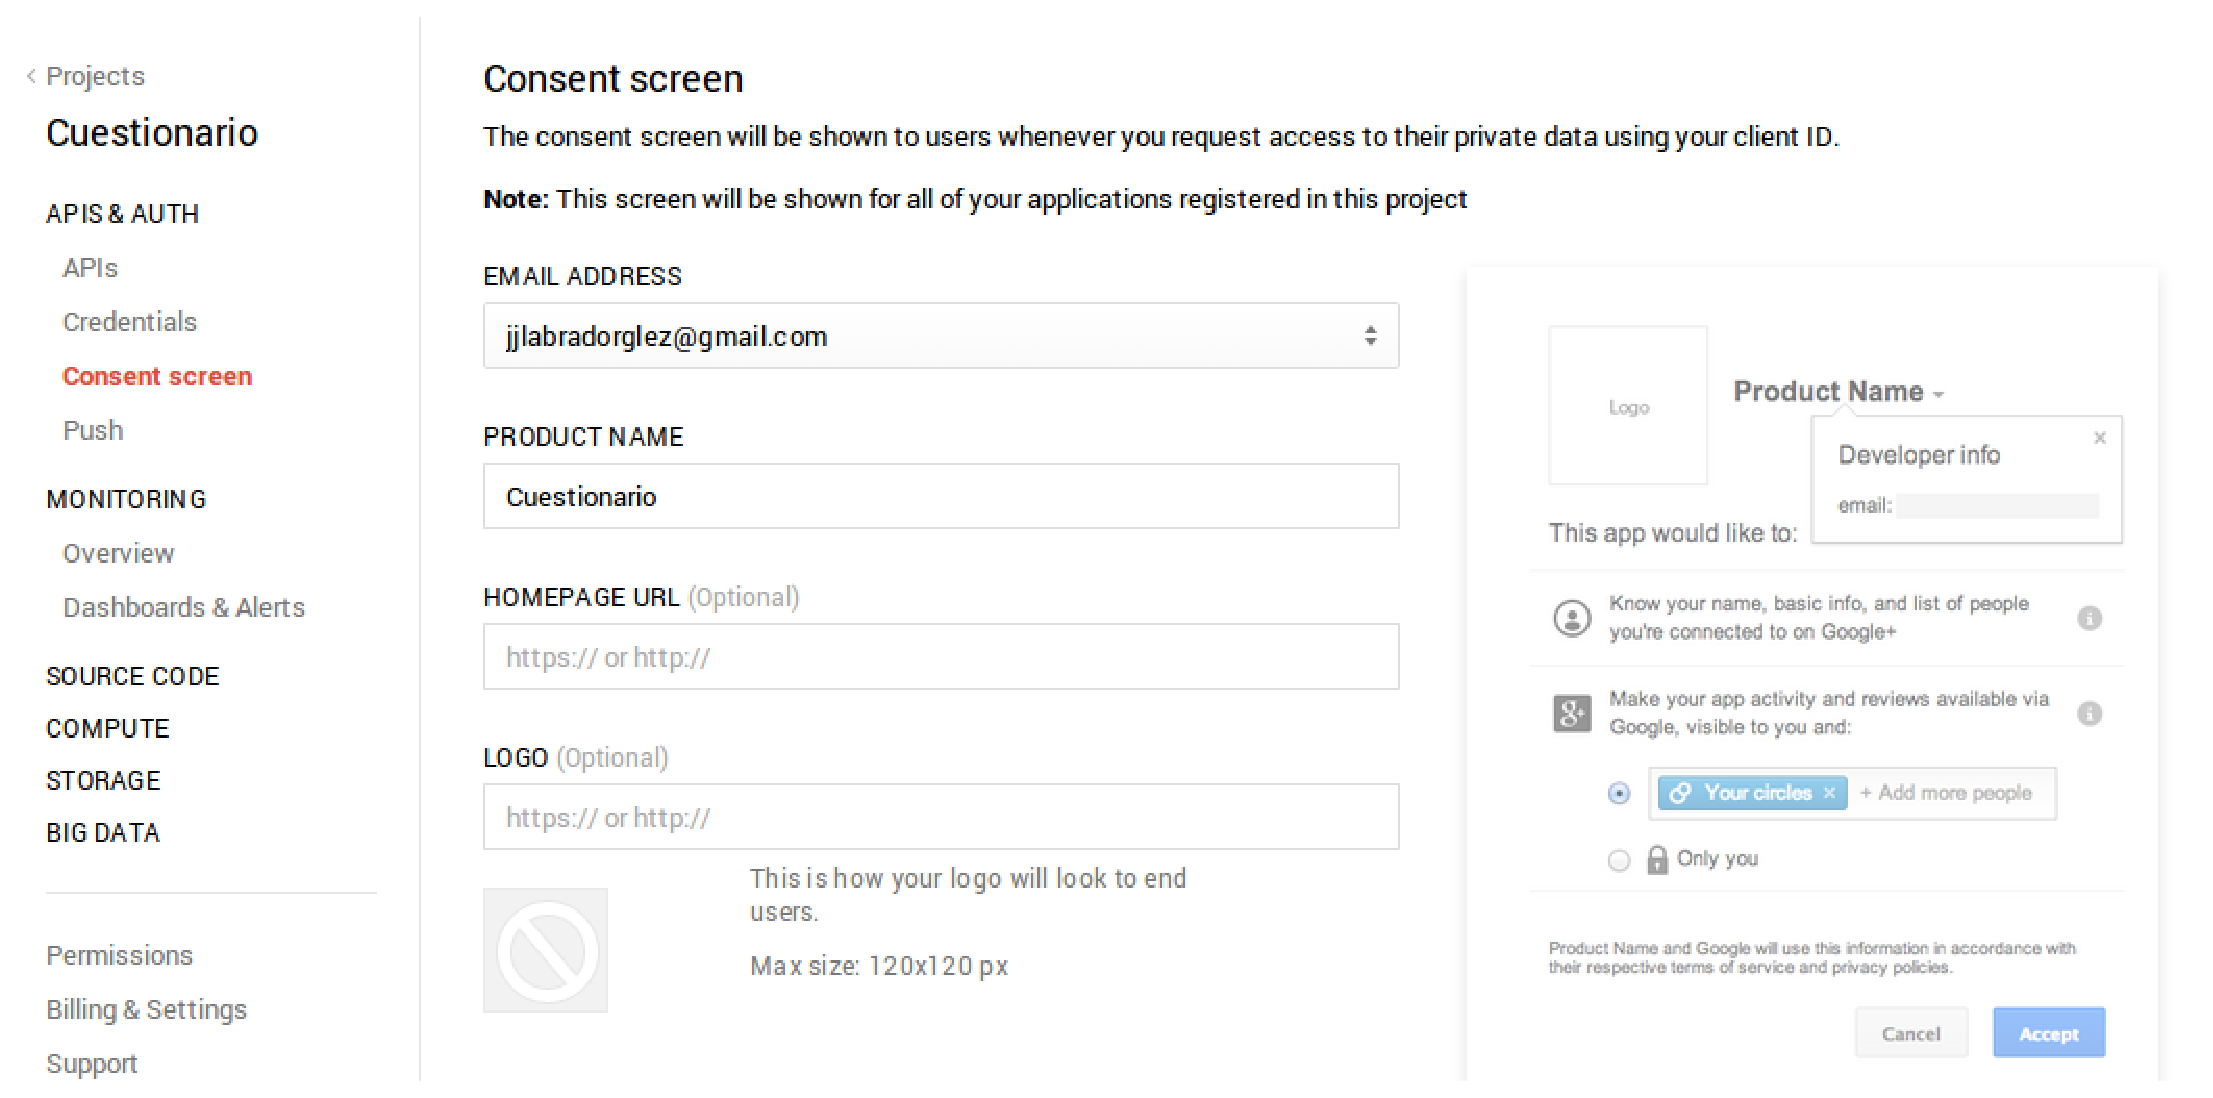
\includegraphics[width=1.2\textwidth]{images/gdc6.eps}
  \caption{Personalizar pantalla de permisos}
  \label{fig:gdc6}
  \end{center}
  \end{figure}
  
\end{enumerate}
\newpage

%---------------------------------------------------------------------------------
\subsection{Generando la aplicaci\'on}
\label{subsec:Apendice2.14}

Para generar la \ceit{aplicaci\'on}, ejecutamos el siguiente comando. Para este renderer es obligatorio el uso de alg\'un template:
\begin{verbatim}
[~]$ ruql [ruta_fichero_rb] Sinatra -t [ruta_template.html.erb]
\end{verbatim}

%---------------------------------------------------------------------------------
\subsection{Ficheros y directorios generados por el renderer}
\label{subsec:Apendice2.15}

Finalmente, los ficheros que genera este renderer son:
\begin{itemize}
  \item El c\'odigo Ruby del servidor ({\bfseries app.rb}).
  \item Un fichero {\bfseries config.ru} para la ejecuci\'on de la aplicaci\'on.
  \item Las vistas necesarias de la aplicaci\'on (incluyendo el cuestionario generado en HTML y un \ceit{template} \ceit{ERB} que se usar\'a para crear las copias de los cuestionarios
  realizados por los alumnos).
  \item Un \ceis{Gemfile} con las dependencias necesarias.
  \item Un \ceis{Rakefile} para automatizar tareas (de ejecuci\'on y despliegue de la aplicaci\'on).
  \item Una carpeta denominada \textit{config} con los datos de alumnos, profesores, las preguntas y respuestas y una copia del fichero \textit{config.yml}
  del cual se hara una lectura de los par\'ametros. De este modo, evitamos que las variables existentes en el c\'odigo contengan la informaci\'on sensible.
\end{itemize}
\newpage

%---------------------------------------------------------------------------------
\subsection{Ejecutando la aplicaci\'on}
\label{subsec:Apendice2.16}

En esta secci\'on se explicar\'a visualmente las funciones que realiza la aplicaci\'on:
\begin{enumerate}
  \item Si el alumno visita el cuestionario antes de que est\'e abierto, ver\'a la siguiente p\'agina:
  \begin{figure}[!th]
  \begin{center}
  
\includegraphics[width=0.9\textwidth]{images/app1.eps}
  \caption{Mensaje anunciando que el cuestionario no est\'a abierto}
  \label{fig:app1}
  \end{center}
  \end{figure}
  
  \item Si el alumno visita el cuestionario despu\'es de que se haya cerrado, ver\'a la siguiente p\'agina:
  \begin{figure}[!th]
  \begin{center}
  
\includegraphics[width=0.9\textwidth]{images/app2.eps}
  \caption{Mensaje anunciando que el cuestionario est\'a cerrado}
  \label{fig:app2}
  \end{center}
  \end{figure}
  \newpage
  
  \item Tanto los alumnos como los profesores ver\'an esta p\'agina al iniciar sesi\'on:
  \begin{figure}[!th]
  \begin{center}
  
\includegraphics[width=0.9\textwidth]{images/app3.eps}
  \caption{P\'agina de iniciar sesi\'on}
  \label{fig:app3}
  \end{center}
  \end{figure}
  
  
  \item El profesor ver\'a esta p\'agina cuando vaya a activar el cuestionario:
  \begin{figure}[!th]
  \begin{center}
  
\includegraphics[width=0.75\textwidth]{images/app4.eps}
  \caption{P\'agina de activar cuestionario}
  \label{fig:app4}
  \end{center}
  \end{figure}
  \newpage
  
  \item Tanto los alumnos como los profesores ver\'an esta p\'agina para dar permisos a la aplicaci\'on al iniciar sesi\'on con \ceit{Google}:
  \begin{figure}[!th]
  \begin{center}
  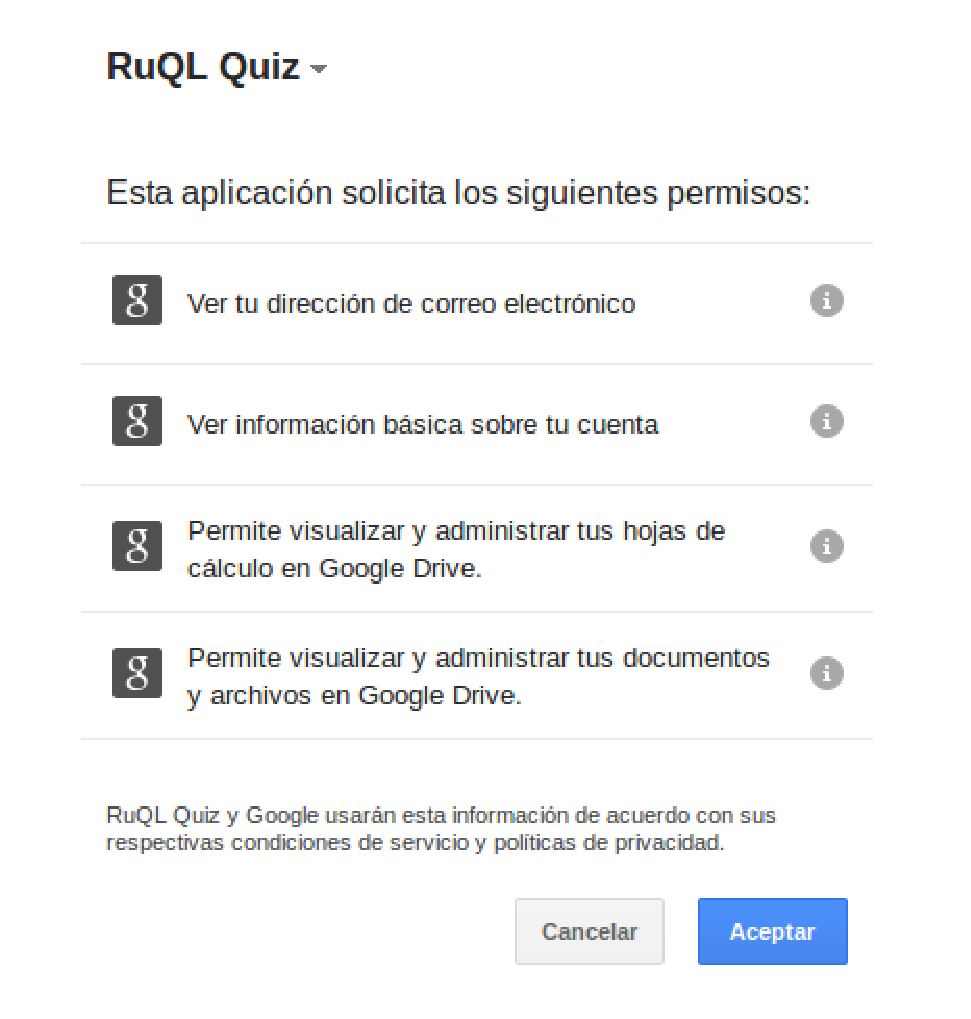
\includegraphics[width=0.6\textwidth]{images/app5.eps}
  \caption{P\'agina de dar permisos a la aplicaci\'on}
  \label{fig:app5}
  \end{center}
  \end{figure}
  
  \item Mientras el profesor no haya activado el \ceit{cuestionario}, los alumnos ver\'an esta p\'agina:
  \begin{figure}[!th]
  \begin{center}
  
\includegraphics[width=0.75\textwidth]{images/app6.eps}
  \caption{Mensaje anunciando que el cuestionario a\'un no est\'a activado}
  \label{fig:app6}
  \end{center}
  \end{figure}
  \newpage
  
  \item Cuando el profesor active el cuestionario ver\'a esta p\'agina. Puede ir a Google Drive para comprobar que la \ceit{hoja de c\'alculo} 
  se ha creado correctamente o visitar el cuestionario desplegado:
  \begin{figure}[!th]
  \begin{center}
  
\includegraphics[width=0.8\textwidth]{images/app7.eps}
  \caption{Mensaje anunciando que el cuestionario ha activado}
  \label{fig:app7}
  \end{center}
  \end{figure}

  \item As\'{\i} se ver\'{\i}a el cuestionario desplegado:
  \begin{figure}[!th]
  \begin{center}
  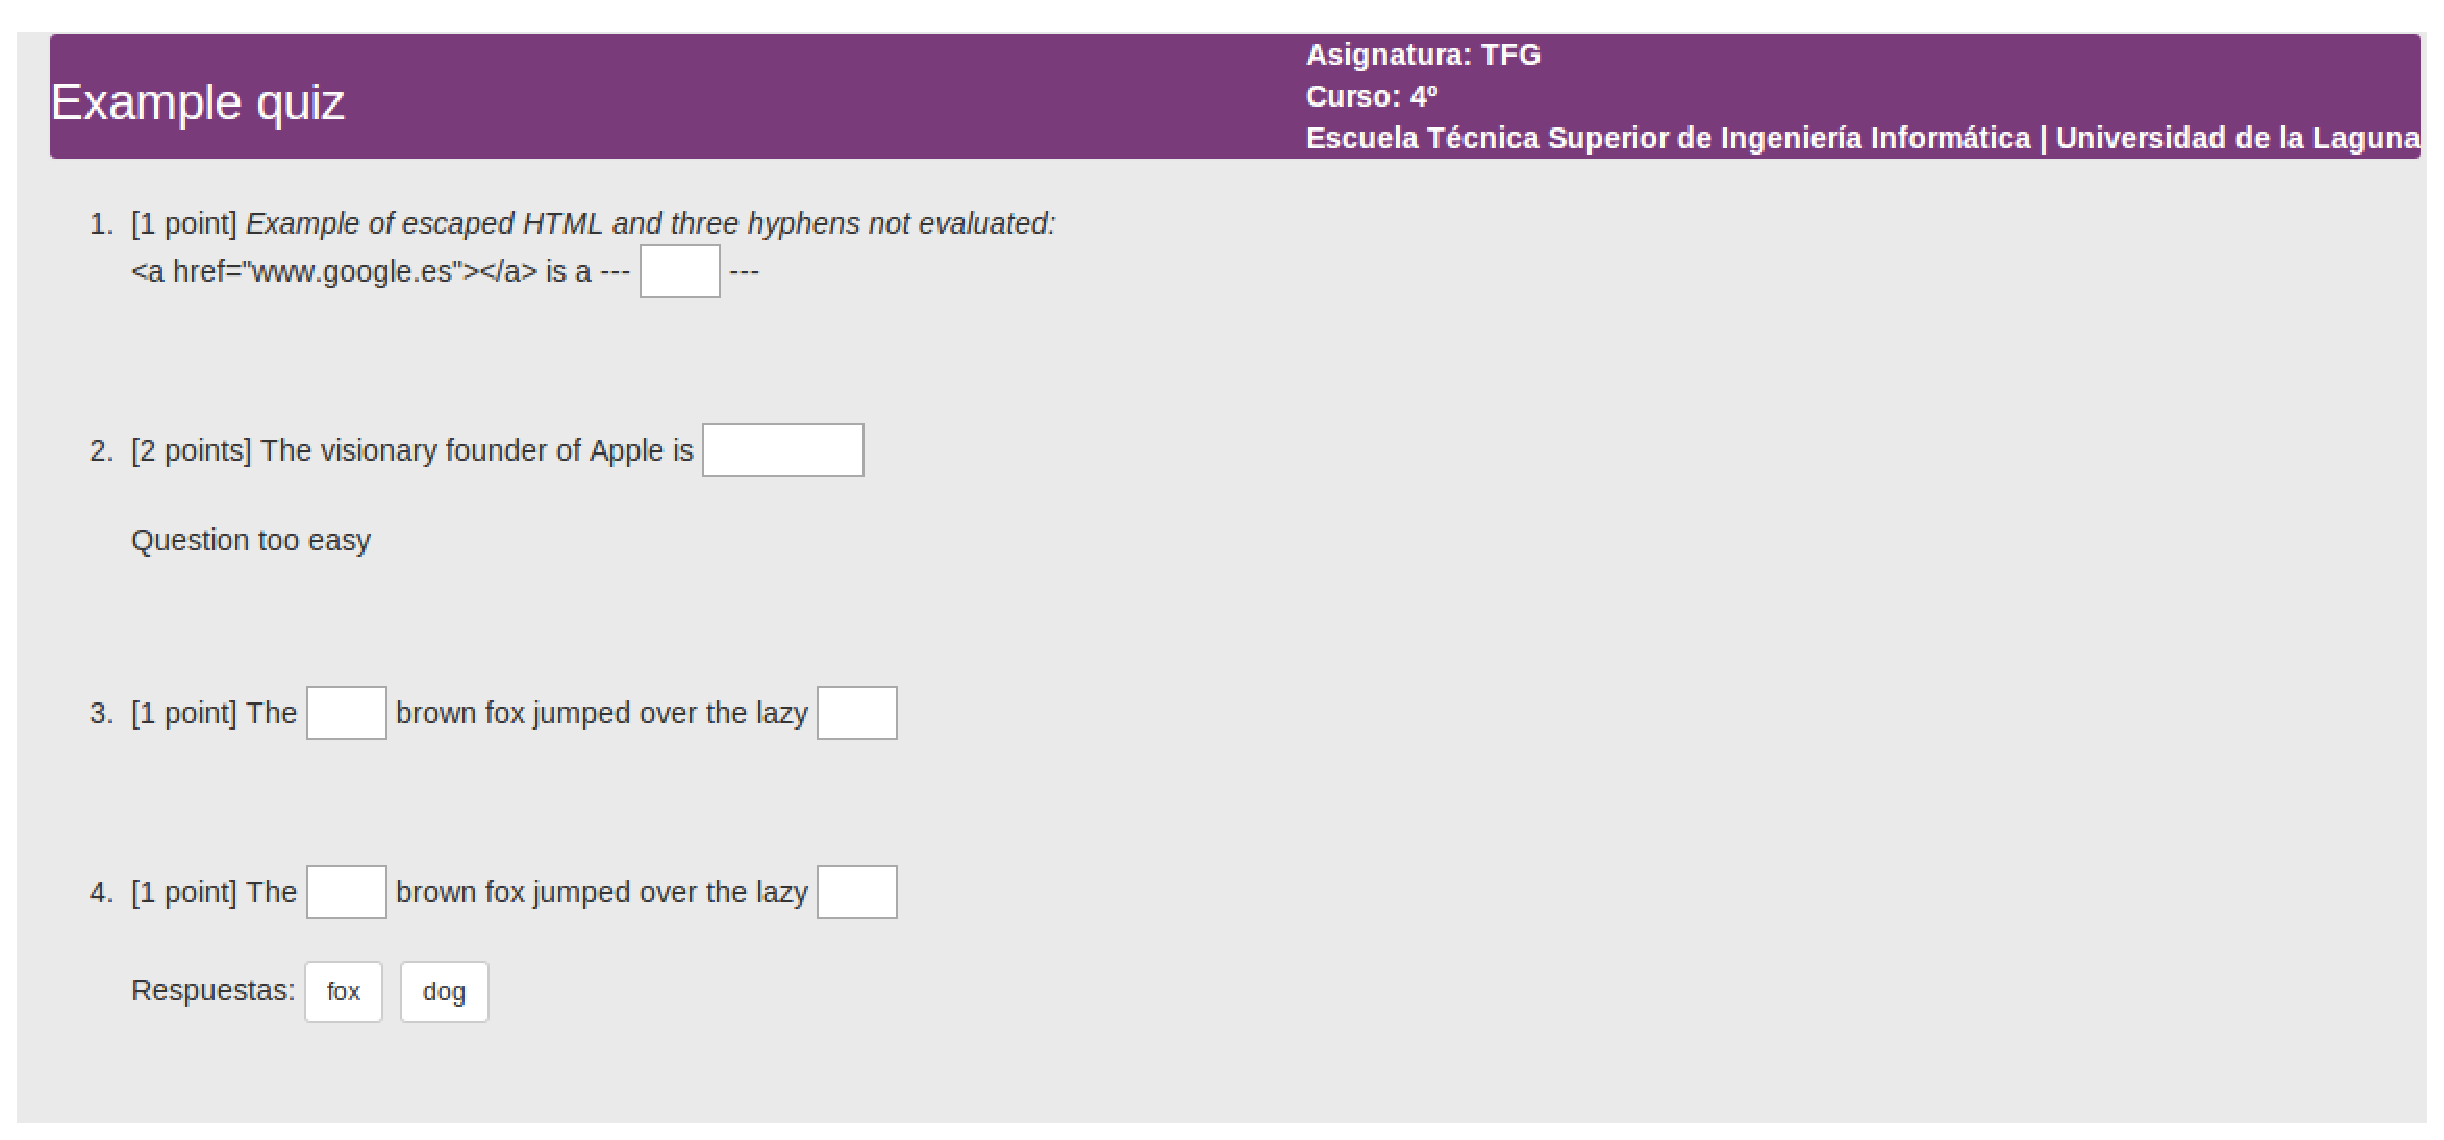
\includegraphics[width=1\textwidth]{images/app8.eps}
  \caption{Cuestionario desplegado}
  \label{fig:app8}
  \end{center}
  \end{figure}
  \newpage
  
  \item Cuando el profesor termine de comprobar el cuestionario y pulse \textit{Enviar}, ver\'a la siguiente pantalla, que le permitir\'a regresar al cuestionario o ver
  su carpeta de Google Drive.
  \begin{figure}[!th]
  \begin{center}
  
\includegraphics[width=0.8\textwidth]{images/app9.eps}
  \caption{Mensaje anunciando que ha finalizado la revisi\'on del cuestionario}
  \label{fig:app9}
  \end{center}
  \end{figure}

  \item Esto es lo que ver\'a el profesor en su carpeta de \ceit{Google Drive}.
  \begin{figure}[!th]
  \begin{center}
  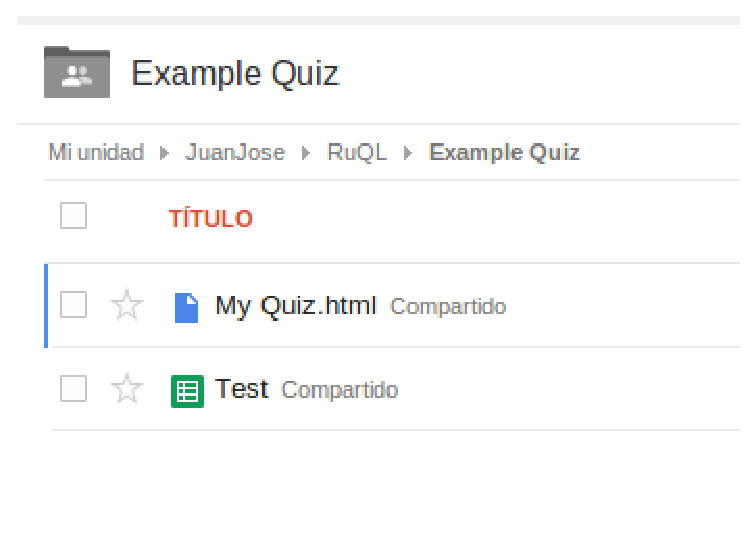
\includegraphics[width=0.6\textwidth]{images/app10.eps}
  \caption{Ficheros dentro de la carpeta del cuestionario en Google Drive}
  \label{fig:app10}
  \end{center}
  \end{figure}
  \newpage

  \item Esta es la hoja de c\'alculo creada con toda la informaci\'on. Esta es la primera hoja, que contiene la informaci\'on de los alumnos.
  \begin{figure}[!th]
  \begin{center}
  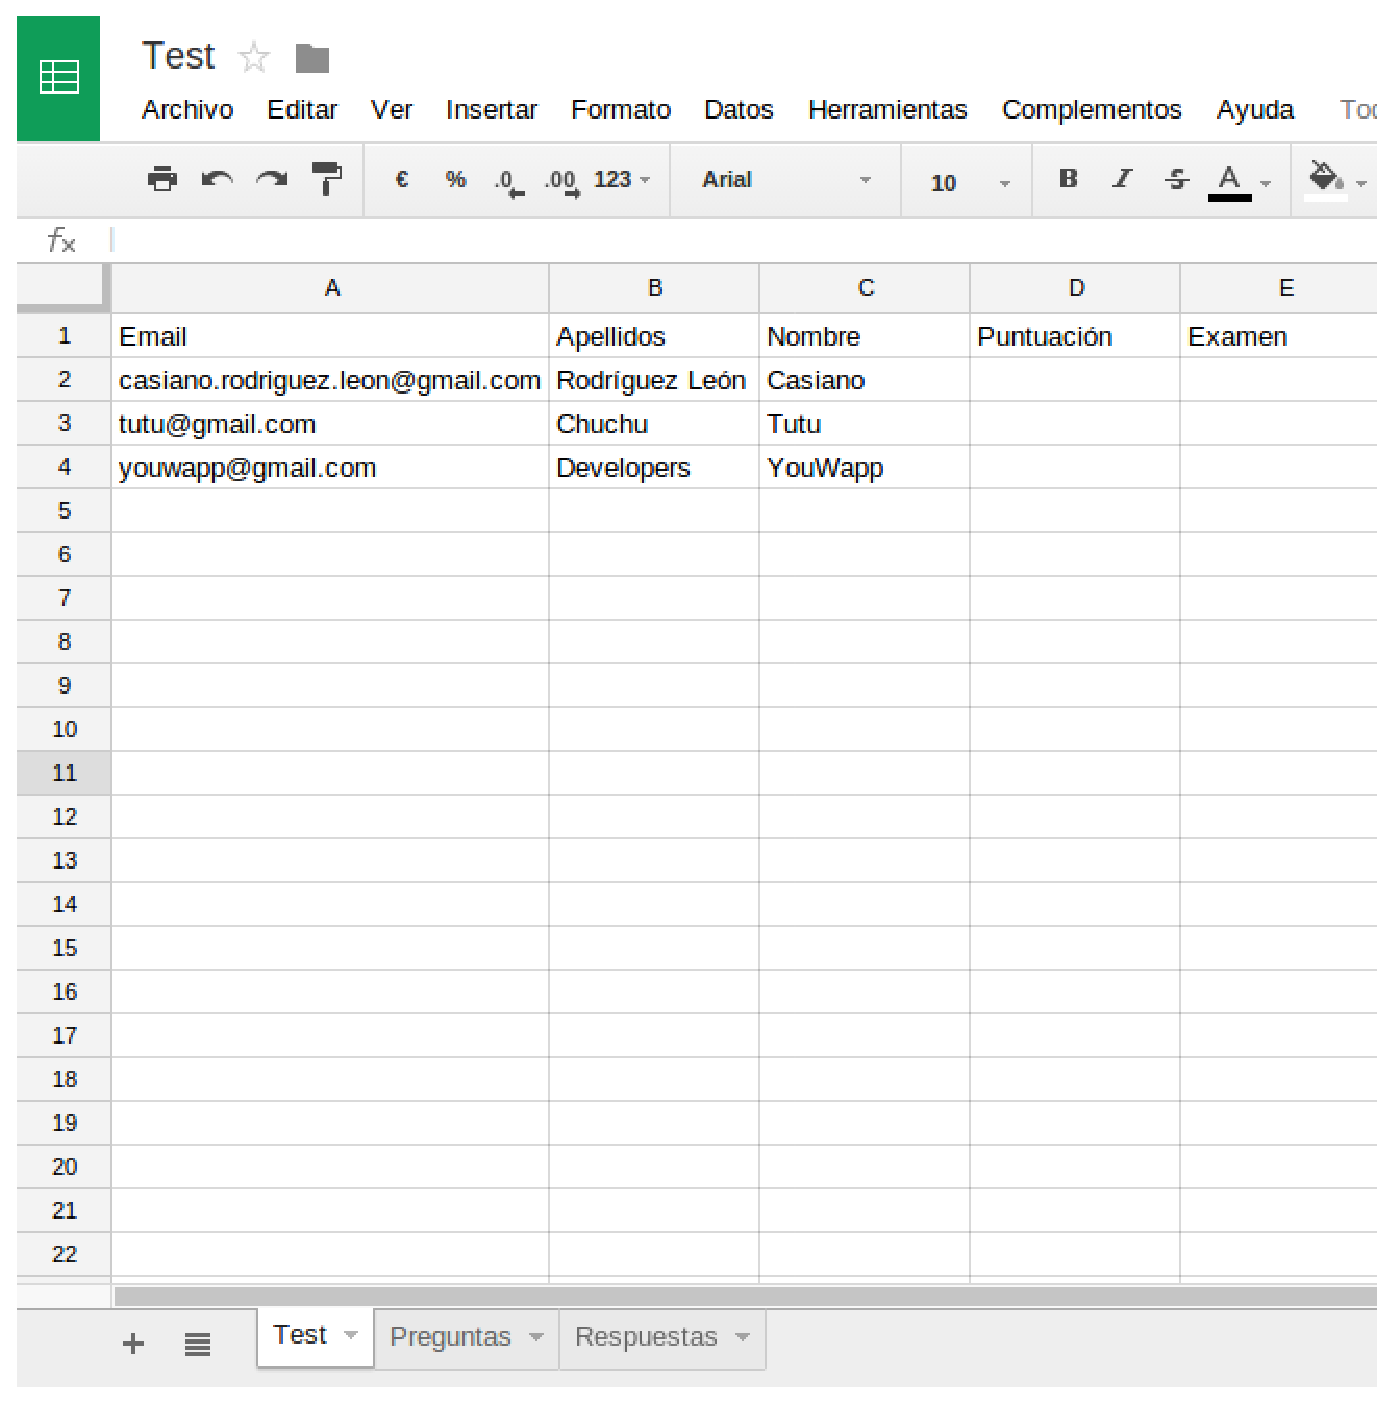
\includegraphics[width=1.1\textwidth]{images/app11.eps}
  \caption{Hoja de c\'alculo con la informaci\'on de los alumnos}
  \label{fig:app11}
  \end{center}
  \end{figure}
  \newpage
  
  \item Esta es la segunda hoja, que contiene la informaci\'on de las preguntas.
  \begin{figure}[!th]
  \begin{center}
  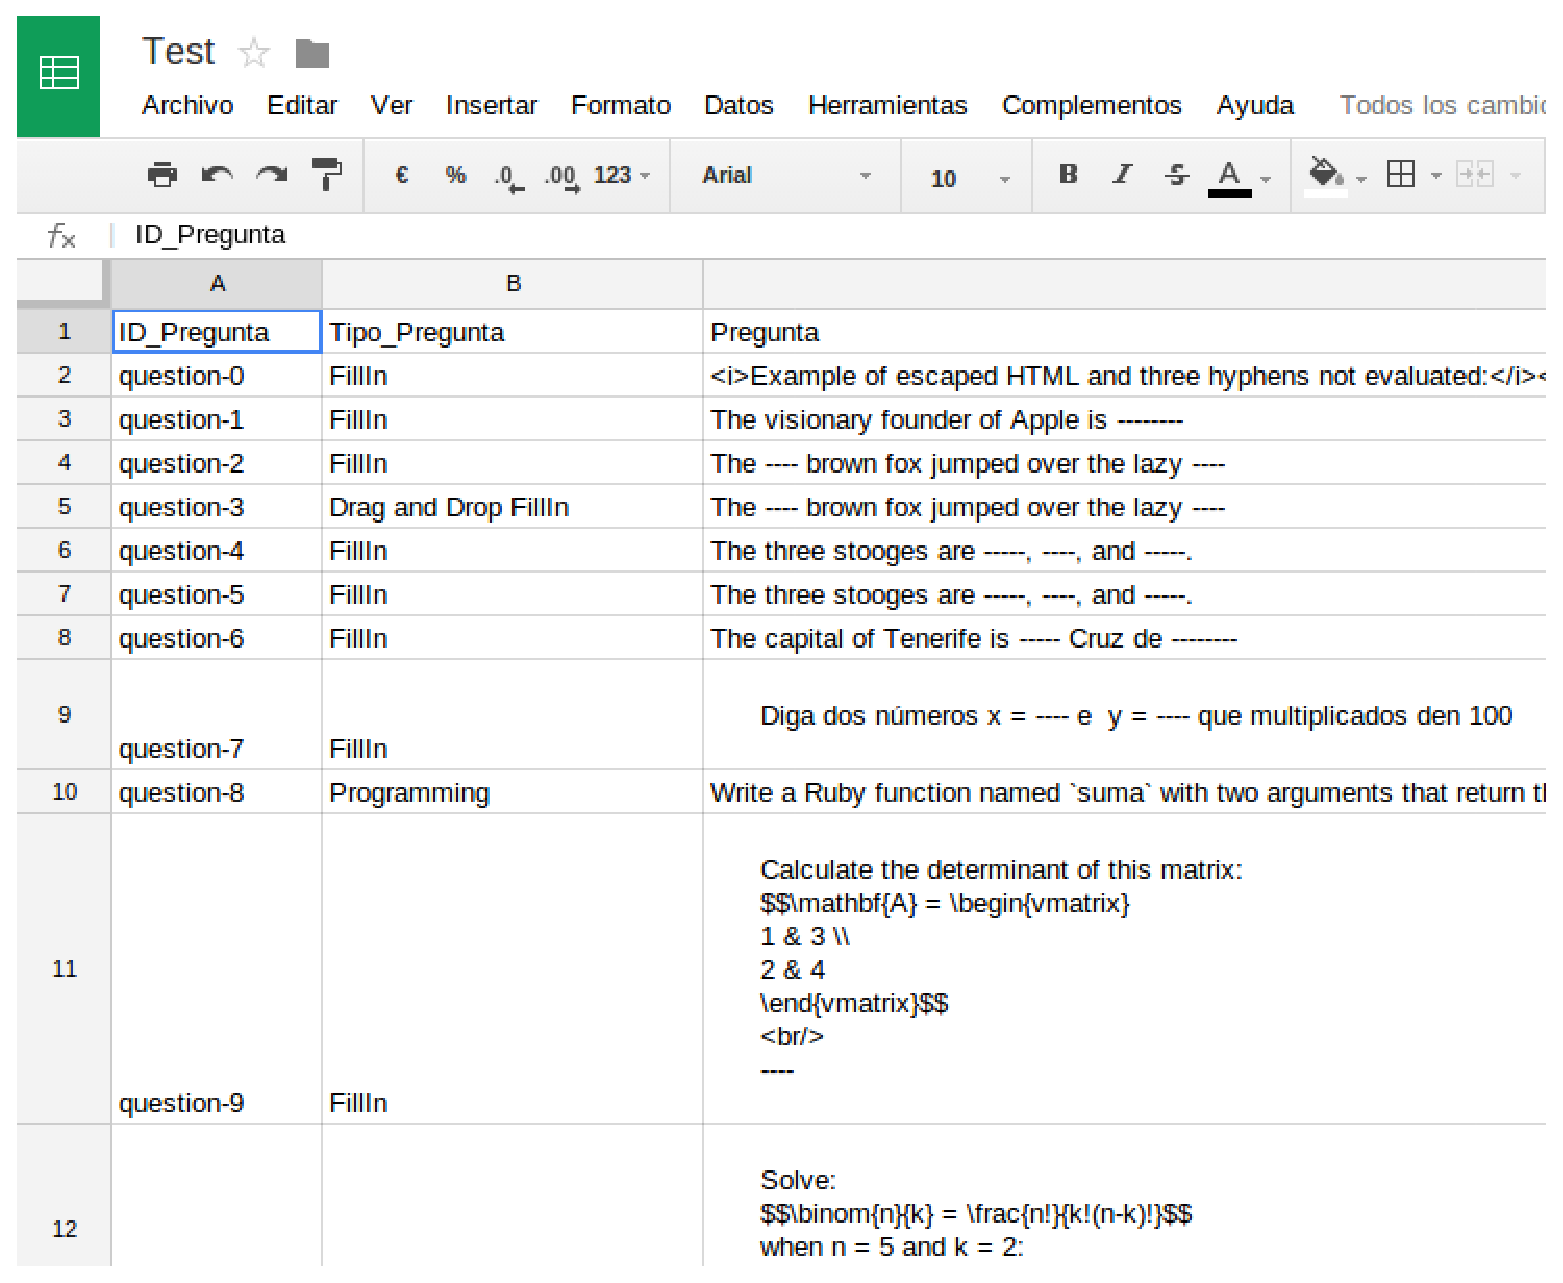
\includegraphics[width=1.1\textwidth]{images/app12.eps}
  \caption{Hoja de c\'alculo con la informaci\'on de las preguntas}
  \label{fig:app12}
  \end{center}
  \end{figure}
  \newpage

  \item Esta es la tercera hoja, que contiene la informaci\'on de las respuestas correctas.
  \begin{figure}[!th]
  \begin{center}
  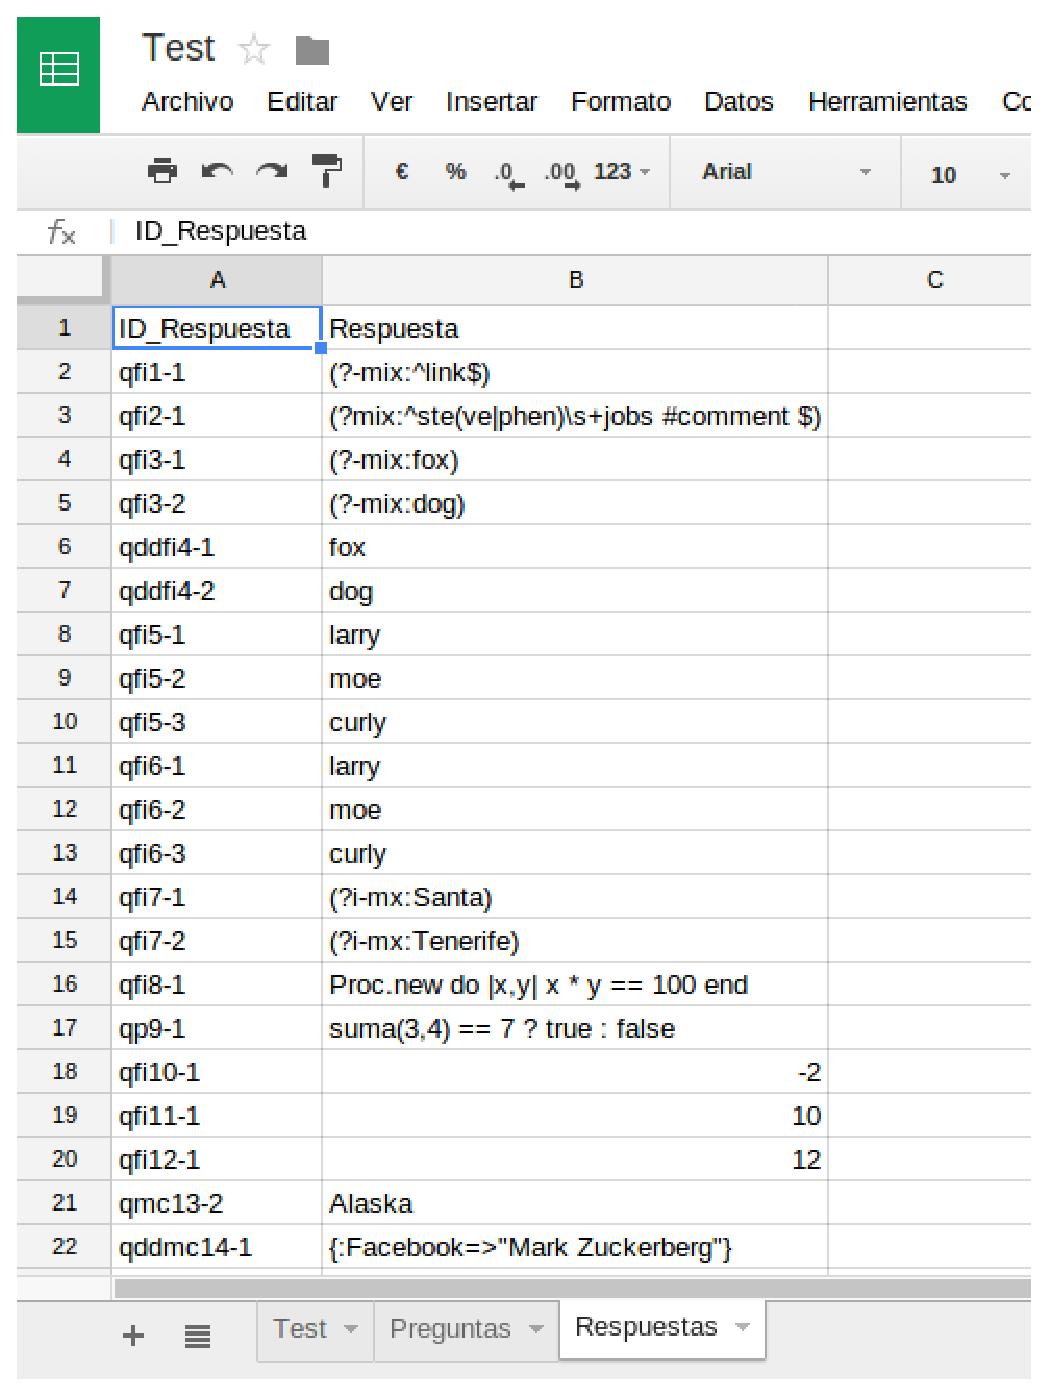
\includegraphics[width=0.8\textwidth]{images/app13.eps}
  \caption{Hoja de c\'alculo con la informaci\'on de las respuestas correctas}
  \label{fig:app13}
  \end{center}
  \end{figure}
  \newpage

  \item Cuando un alumno complete el cuestionario, ver\'a la siguiente pantalla. Podr\'a repetir el cuestionario todas las veces que desee dentro de la
  fecha permitida:
  \begin{figure}[!th]
  \begin{center}
  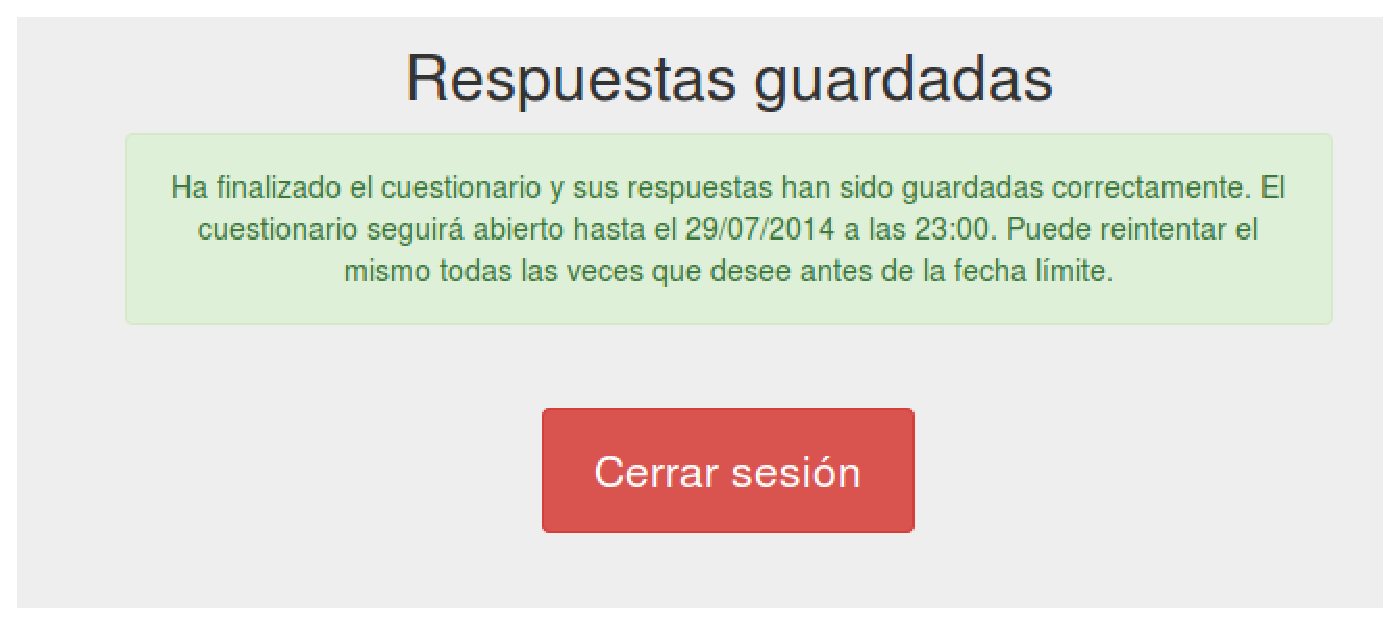
\includegraphics[width=1\textwidth]{images/app14.eps}
  \caption{Mensaje anunciando que ha completado cuestionario}
  \label{fig:app14}
  \end{center}
  \end{figure}
  \newpage
  
  \item Una vez completado el cuestionario, se crear\'a una nueva hoja dentro de la hoja de c\'alculo del profesor con la puntuaci\'on que ha
  sacado el alumno en cada pregunta:
  \begin{figure}[!th]
  \begin{center}
  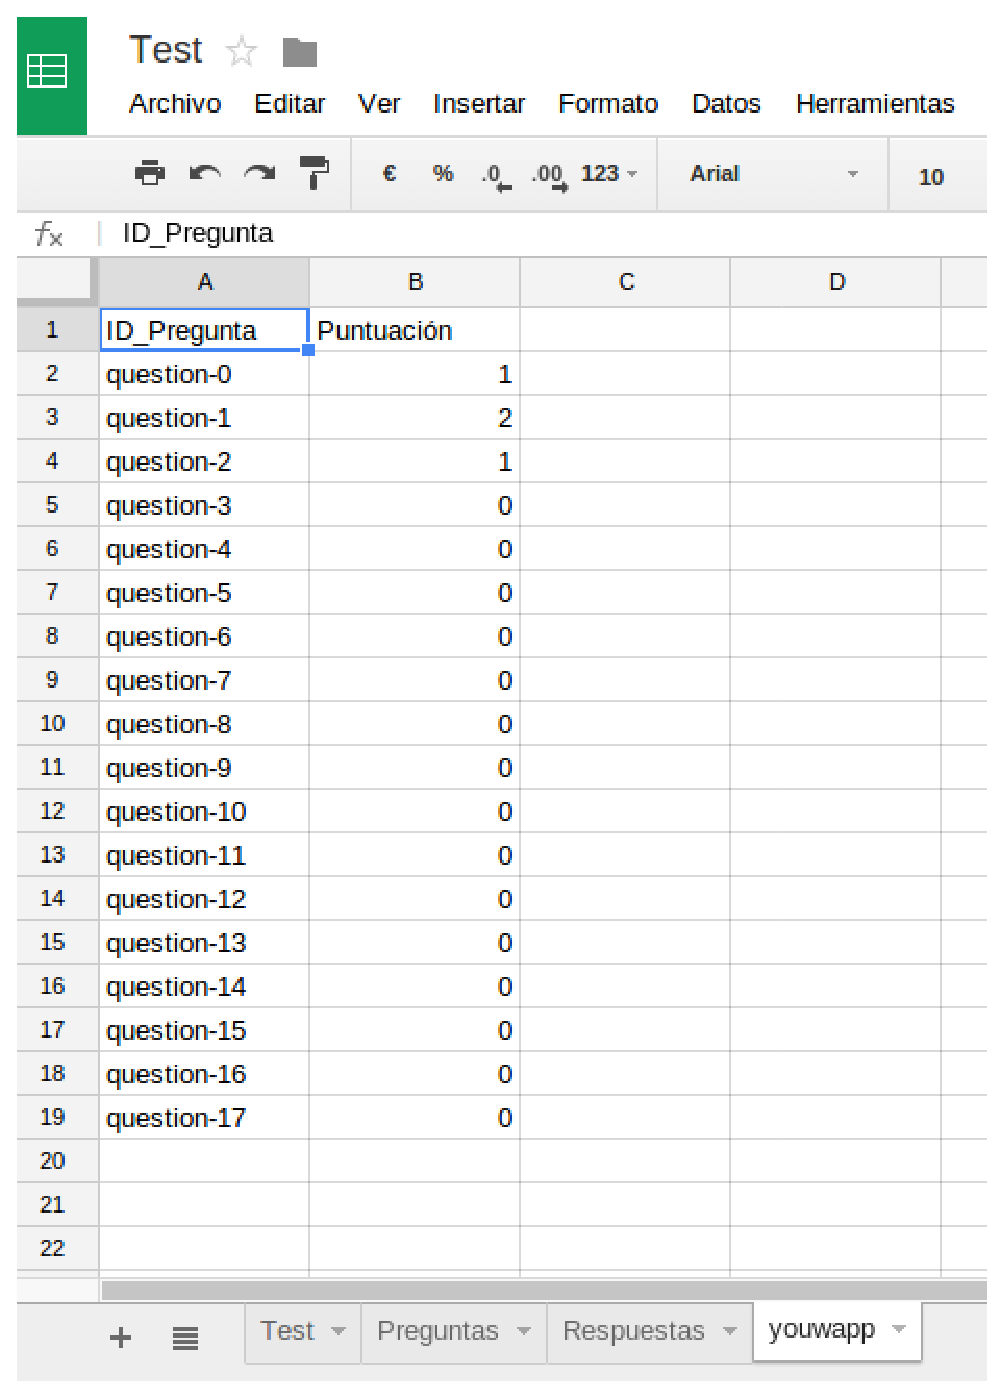
\includegraphics[width=0.8\textwidth]{images/app15.eps}
  \caption{Hoja de c\'alculo con la puntuaci\'on por preguntas}
  \label{fig:app15}
  \end{center}
  \end{figure}
  \newpage
  
  \item En la primera hoja, se a\~{n}adir\'a la informaci\'on del alumno que hizo el cuestionario, su nota y un enlace a la copia del \ceit{examen} que realiz\'o.
  \begin{figure}[!th]
  \begin{center}
  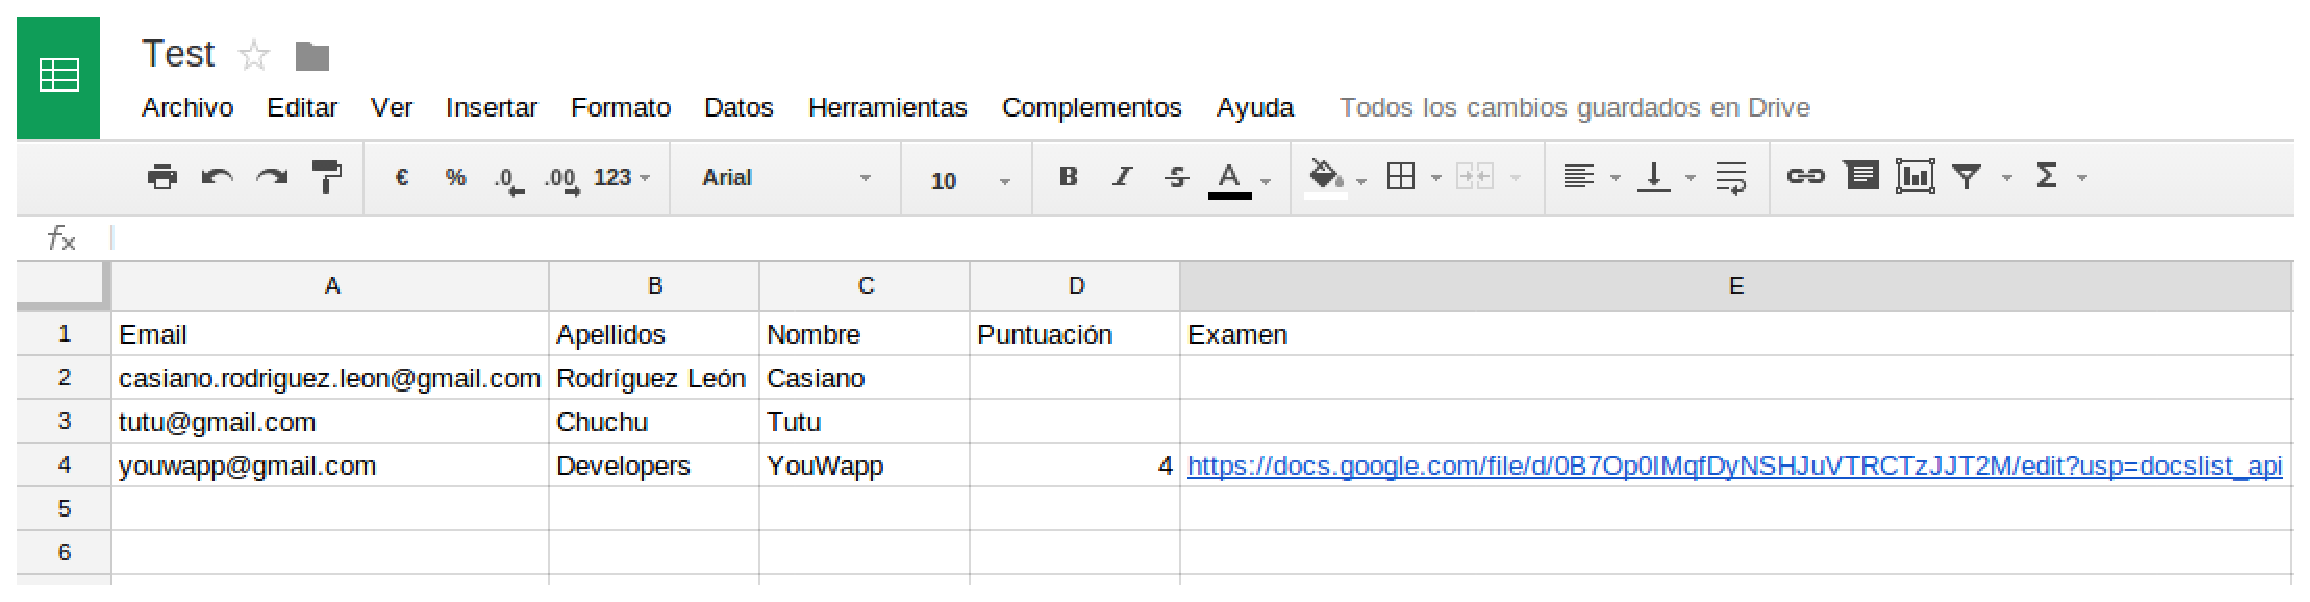
\includegraphics[width=1.1\textwidth]{images/app16.eps}
  \caption{Informaci\'on actualizada del alumno que realiz\'o el cuestionario}
  \label{fig:app16}
  \end{center}
  \end{figure}
  
  \item Dentro de la carpeta de Google Drive del profesor se crear\'a, adem\'as, una copia del cuestionario con las respuestas que puso el alumno.
  \begin{figure}[!th]
  \begin{center}
  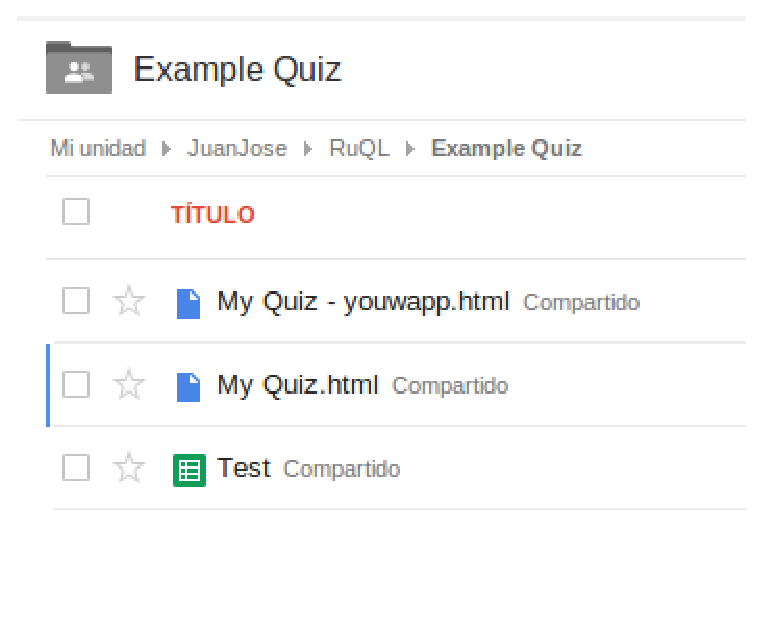
\includegraphics[width=0.6\textwidth]{images/app17.eps}
  \caption{Listado de ficheros en Google Drive con la copia hecha por el alumno}
  \label{fig:app17}
  \end{center}
  \end{figure}
  \newpage
  
  \item Por \'ultimo, esta ser\'{\i}a la copia del cuestionario generada con las respuestas del alumno:
  \begin{figure}[!th]
  \begin{center}
  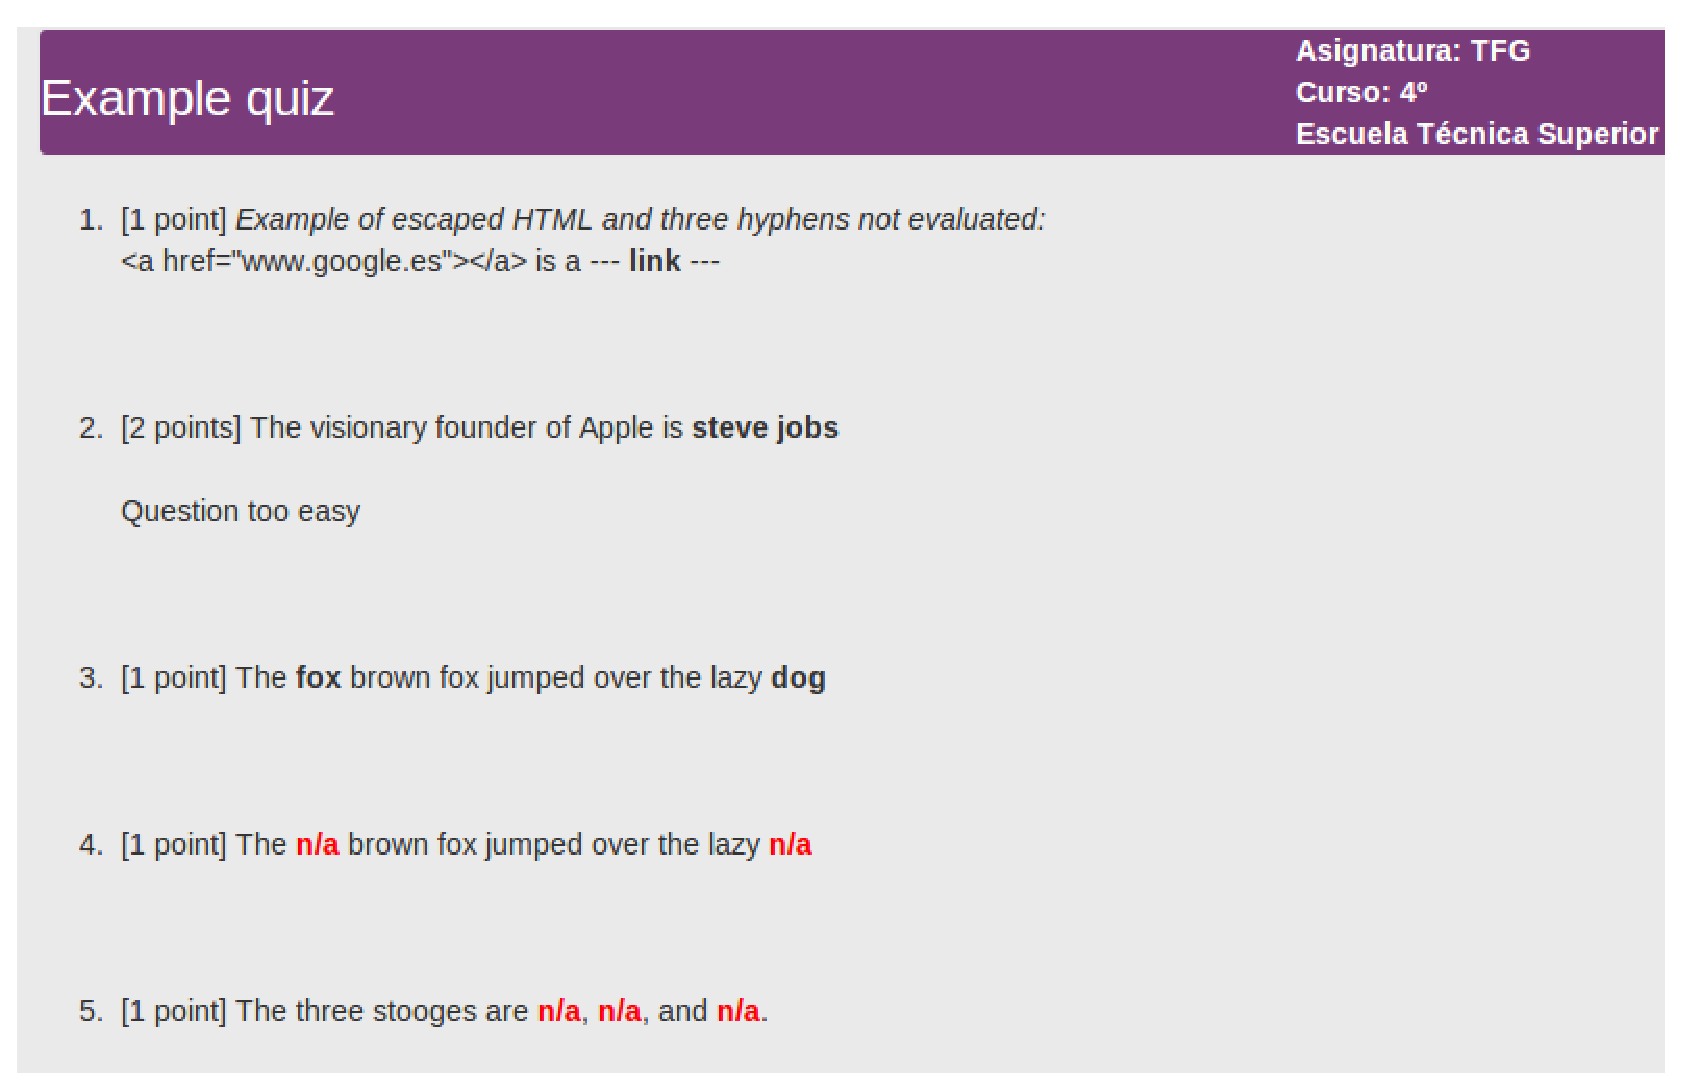
\includegraphics[width=1\textwidth]{images/app18.eps}
  \caption{Copia del cuestionario con las respuestas del alumno}
  \label{fig:app18}
  \end{center}
  \end{figure}
  
\end{enumerate}

%---------------------------------------------------------------------------------
\subsection{Otras consideraciones}
\label{subsec:Apendice2.17}

\begin{itemize}
  \item Este renderer no permite la opci\'on de mostrar respuestas mientras se realiza el cuestionario.
  \item El \ceit{Local Storage} tambi\'en funciona en este renderer, sin embargo, al ser un \ceit{JavaScript}, el evento de guardado de respuestas se dispara al perder el foco
  el \ceit{input} o \ceit{textarea} en el que nos encontramos.
\end{itemize}